\section{Result}

\begin{figure}[H]
    \centering
    \begin{subfigure}[b]{0.99\textwidth} 
        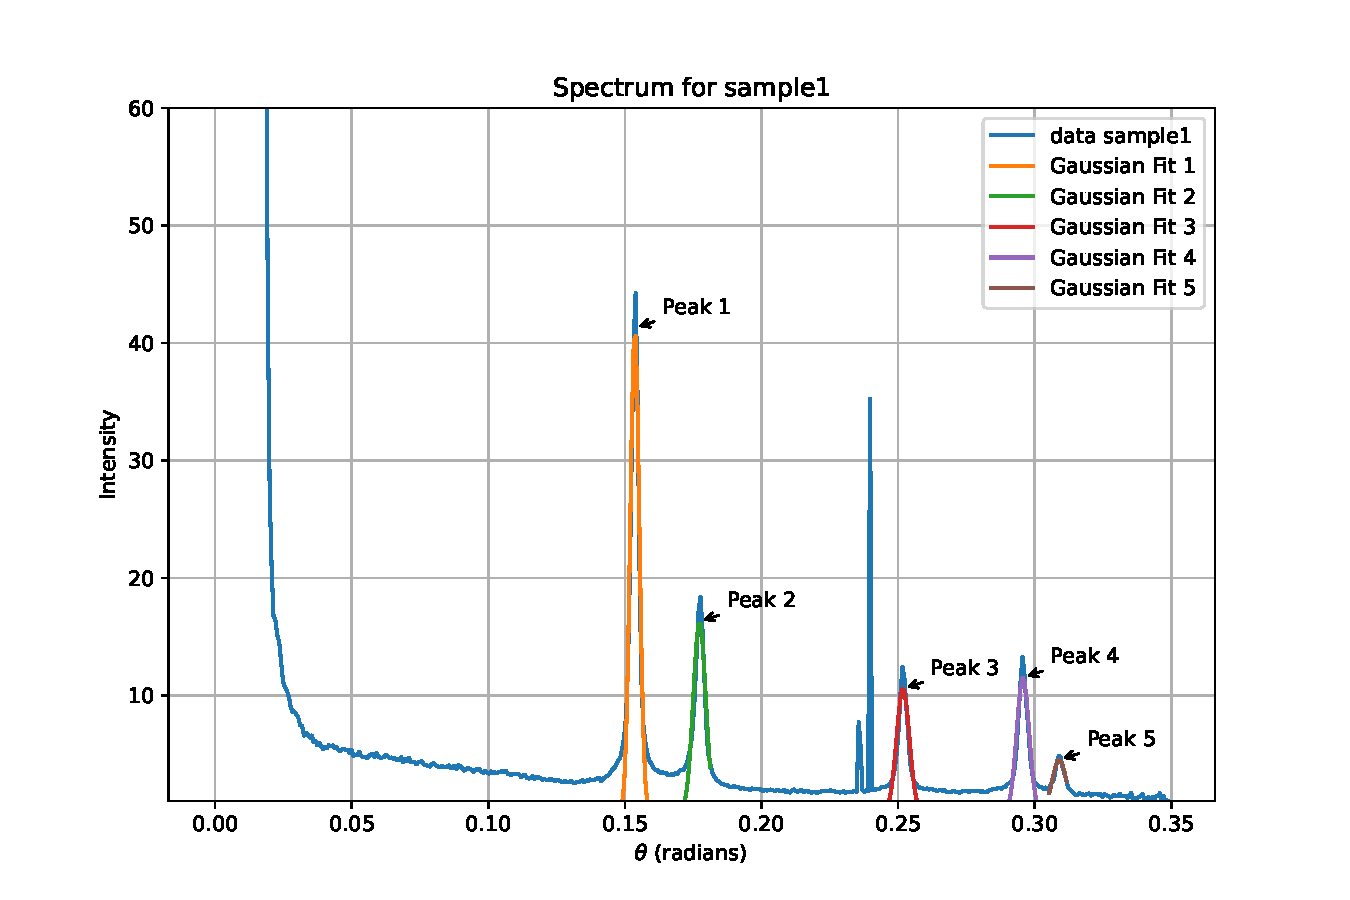
\includegraphics[width=\textwidth]{Figures/gaussian_sample1.pdf}
        \subcaption{This is the first subfigure.}
        \label{fig:subfigure1}
    \end{subfigure}
    \begin{subfigure}[b]{0.99\textwidth} 
        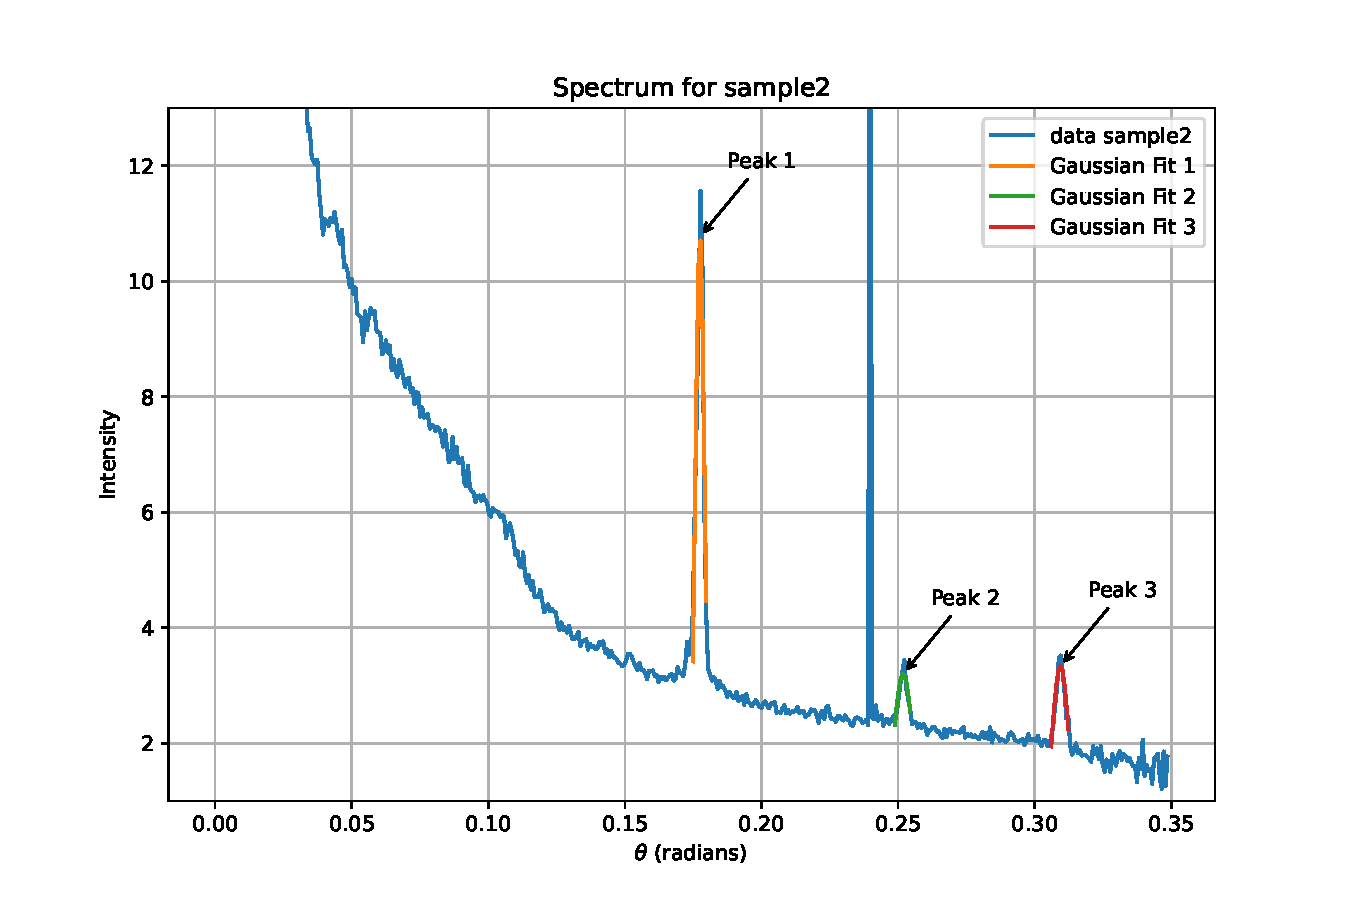
\includegraphics[width=\textwidth]{Figures/gaussian_sample2.pdf}
        \subcaption{This is the second subfigure.}
        \label{fig:subfigure2}
    \end{subfigure}
    \caption{This figure shows two subfigures with separate captions.}
    \label{fig:result_figure}
\end{figure}

\begin{enumerate}
    \item For sample1:
    \begin{enumerate}
    \item Peak 1: Amplitude = 41.29 $\pm$ 2.15 (units), Mean = 0.15362 $\pm$ 0.00010 (radians), Sigma = 0.00165 $\pm$ 0.00010 (radians), FWHM = 0.00388 $\pm$ 0.00023 (radians)
    \item Peak 2: Amplitude = 16.28 $\pm$ 1.14 (units), Mean = 0.17731 $\pm$ 0.00019 (radians), Sigma = 0.00227 $\pm$ 0.00020 (radians), FWHM = 0.00535 $\pm$ 0.00046 (radians)
    \item Peak 3: Amplitude = 10.57 $\pm$ 0.71 (units), Mean = 0.25180 $\pm$ 0.00018 (radians), Sigma = 0.00234 $\pm$ 0.00018 (radians), FWHM = 0.00550 $\pm$ 0.00043 (radians)
    \item Peak 4: Amplitude = 11.53 $\pm$ 0.66 (units), Mean = 0.29569 $\pm$ 0.00015 (radians), Sigma = 0.00225 $\pm$ 0.00015 (radians), FWHM = 0.00530 $\pm$ 0.00035 (radians)
    \item Peak 5: Amplitude = 4.51 $\pm$ 0.19 (units), Mean = 0.30900 $\pm$ 0.00015 (radians), Sigma = 0.00261 $\pm$ 0.00021 (radians), FWHM = 0.00616 $\pm$ 0.00049 (radians)
    \end{enumerate}
    \end{enumerate}
    \begin{enumerate}
    \item For sample2:
    \begin{enumerate}
    \item Peak 1: Amplitude = 10.77 $\pm$ 0.62 (units), Mean = 0.17746 $\pm$ 0.00012 (radians), Sigma = 0.00172 $\pm$ 0.00014 (radians), FWHM = 0.00404 $\pm$ 0.00034 (radians)
    \item Peak 2: Amplitude = 3.20 $\pm$ 0.09 (units), Mean = 0.25186 $\pm$ 0.00017 (radians), Sigma = 0.00380 $\pm$ 0.00039 (radians), FWHM = 0.00895 $\pm$ 0.00092 (radians)
    \item Peak 3: Amplitude = 3.34 $\pm$ 0.10 (units), Mean = 0.30942 $\pm$ 0.00014 (radians), Sigma = 0.00326 $\pm$ 0.00024 (radians), FWHM = 0.00768 $\pm$ 0.00056 (radians)
    \end{enumerate}
    \end{enumerate}